%$$$$$$$$$$$$$$$$$$$$$$$$$$$$$$$$$$$$$$$$$$$$$$$$$$$$$$$$$$$$$$$$$$$$$$$$$$$$$$$$
%Paragraph 1:Linux Scalability의 연구에 대한 설명
%$$$$$$$$$$$$$$$$$$$$$$$$$$$$$$$$$$$$$$$$$$$$$$$$$$$$$$$$$$$$$$$$$$$$$$$$$$$$$$$$

\newpage
\section{최근 운영체제 병렬화 연구}
\label{sec:osrelated}

%To improve the scalability, researchers have attempted to create new
%operating systems~\cite{Boyd-WickizerCorey}~\cite{Wentzlaff2010fOS}
%~\cite{Baumann2009Barrelfish}~\cite{Zellweger2014Multikernel}
%~\cite{Liu2009Tessellation}~\cite{Farrington2010Helios}
%or have
% attempted to optimize existing operating
%
 % systems~\cite{SilasBoydWickizer2010LinuxScales48}~\cite{AustinTClements2012RCUBalancedTrees}~\cite{Clements2013RadixVM}~\cite{SilasBoydWickizerPth} ~\cite{Changwoo2016UMSF}.
 
코어 수가 증가 되는 상황에서 병렬 화가 중요해진 운영체제에 대한 연구는 성능에
 대한 확장성을 향상 시키기 위해서, 새로운 확장성 있는
운영 체제를 만들거나 ~\cite{Boyd-WickizerCorey}~\cite{Wentzlaff2010fOS}
~\cite{Baumann2009Barrelfish}
~\cite{Liu2009Tessellation}~\cite{Farrington2010Helios} 
기존 운영체제를 최적화 시키는
방법~\cite{SilasBoydWickizer2010LinuxScales48}
~\cite{AustinTClements2012RCUBalancedTrees}~\cite{Clements2013RadixVM}~\cite{SilasBoydWickizerPth}을
시도하고 있다.

\subsection{새로운 운영체제 제안}

%Our research belongs to optimizing existing operating systems in order to
%solve the Linux fork scalability problem.
%이 중 우리의 연구는 리눅스의 fork에 대한 확장성을 개선하기 위한
% 기존 운영체제를 최적화 하는 방법에 속한다. 
%However, previous research did not deal with the anonymous reverse mapping,
%which is one of the fork scalability bottleneck.
%하지만 기존 연구들은 fork의 확장성 병목 지점 중 하나인 익명 역 매핑에 대해서는 처리하지 않았다.

%Cache-line fetches are expensive
%Read cache line written by
%another core: expensive!
%100–10000 cycles
%(contention)

%For reference, a creat system call costs 2.5K cycles
%Avoiding cache-line sharing is challenging
%Consider read-write lock
%struct readwritelock {
%int count;
%// -1, write mode; > 0, read mode
%listhead waiters;
%%spinlock waitlock;
%}
%Problem: to acquire lock in read mode requires modifying count
%%Fetching a remote cache line is expensive
%Many readers can cause performance collapse

\subsubsection{Corey}

Corey~\cite{Boyd-WickizerCorey}는 MIT의 Parallel and Distributed Operating Systems
Group에서 개발하였다.
기본적인 철학은 커널 영역의 공유 데이터를 유저 응용프로그램이 사용할 수 있게 만들어 주어서, 
공유 데이터 때문에 발생하는 경합 문제를 유저에게 해결할 수 있도록 공유에 대한 인터페이스를 제공하는 것이다. 
그 이유는 프로세서 내의 코어 간의 캐시 일관성 작업 때문에 성능이 저하되는데 이러한 것의 원인을 
운영체제가 응용프로그램과는 상관 없이 데이터를 공유하고 하드웨어 역시 응용프로그램에 상관없이 동기화 하는 
방식을 사용하기 때문에 기존의 운영체제에서 취하는 방법은 매니코어 환경에서 성능 향상이 어렵다는 것이다.  
이러한 문제를 해결하기 위해 응용프로그램의 워크로드에 따라 공유 문제를 해결할 수 있는 방향을 제공해준다.
이것은 exokernel[]의 개념을 가져와서 매니코어 시스템에 적용하였고, 이를 통해 확장성을 개선하였다.

%$$$$$$$$$$$$$$$$$$$$$$$$$$$$$$$$$$$$$$$$$$$$$$$$$$$$$$$$$$$$$$$$$$$$$$$$$$$$$$$$
%Paragraph 2:Corey의 3가지 기본 개념 설명
%$$$$$$$$$$$$$$$$$$$$$$$$$$$$$$$$$$$$$$$$$$$$$$$$$$$$$$$$$$$$$$$$$$$$$$$$$$$$$$$$
이러한 Corey는 3가지 기본적은 개념을 가지고 있다. 그것은 address rages, 커널 kernel core 그리고 shares이다.
첫째로, address rages는 운영체제의 스레드간의 공유하는 데이터인 address space에 대해서 다룬다.
대부분의 운영체제는 address space를 space를 그림~\ref{fig:corey}(a)와 같이 single address space로
구성하는 경우와  그림~\ref{fig:corey}(b)와 같이 per-core 기반의 separate address space로 구성된다.
만약 single address space를 사용할 경우 모든 코어가 같은 address space를 사용함에 따라 반드시 락이 필요하다.
따라서 예를들어, 맵리듀스와 같은 응용프로그램을 사용할 경우 맵 단계에서 굉장히 많은 락 경합이 발생하게 된다.
또한, 만약 separate address space를 사용할 경우 리듀스 단계에서 공유하지 않은 데이터에 접급함에 따라
soft page fault가 많이 발생하는 문제가 있다.
Corey는 이러한 문제를 address rages라는 개념으로 해결하였다. 
이것은 separate address space를 제공함과 동시에 중간 결과를 공유할 수 있는 방법을 제공함으로 single address
space의 장점을 동시에 취한다.
다음으로, kernel core는 응용프로그램을 공유 메모리를 사용하지 않고, 특정 코어에 
독점 할당 시켜주고 공유는 IPC로 하도록 제공하는 기술이다. 
따라서 스케줄러와 인터럽트등에 방해을 받지 않고 캐시 지역성을 높여 성능을 향상 시키는 방법이다.
마지막으로, 공유는 어떻게 커널 자료구조를 접근할 수 있는 지에 대해서 제공해준다.

\begin{figure}[h!]
    \centering
    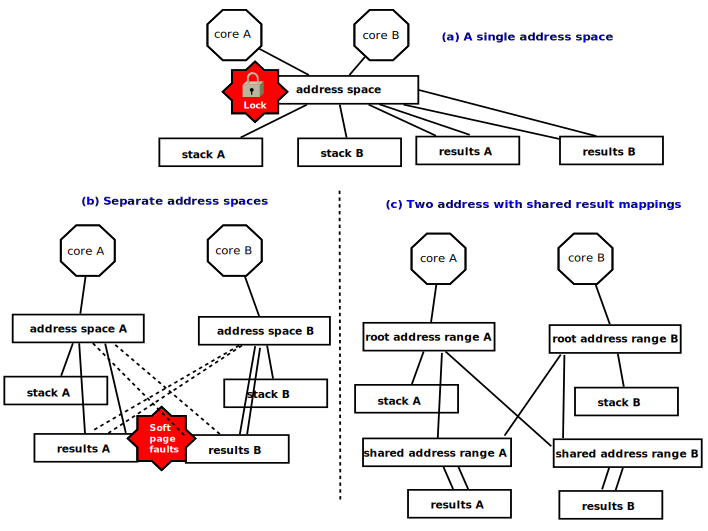
\includegraphics[width=1\textwidth]{fig/corey/corey}
    \caption{corey 운영체제 address space 공유 방법}
  \label{fig:corey}
\end{figure}

\subsubsection{Barrelfish}

%$$$$$$$$$$$$$$$$$$$$$$$$$$$$$$$$$$$$$$$$$$$$$$$$$$$$$$$$$$$$$$$$$$$$$$$$$$$$$$$$
%Paragraph : Barrelfish의 특징 설명
%$$$$$$$$$$$$$$$$$$$$$$$$$$$$$$$$$$$$$$$$$$$$$$$$$$$$$$$$$$$$$$$$$$$$$$$$$$$$$$$$

Barrelfish~\cite{Baumann2009Barrelfish}는 취히리의 ETH와 마이크로 소프트(Microsoft)가
공동 연구하여 만든 운영체제이다.
Barrelfish는 멀티커널(multikernel) 운영체제 중 하나 이고, 기본적인 철학은 공유 메모리 시스템 
기능들을 모두 분산 처리 방식으로 구현하자는 것이다.
예를 들어, 운영체제에서 각 코어는 네트워크로 분산 된 시스템으로 가정하고 메시지 패싱을 통해 분산 된 
코어들 간에 통신을 하여, 성능을 향상 시킨 방법이다. 
메시지 패싱 방법을 사용한 이유는, 오늘날 사용되는 캐시 구조로 된 시스템의 
single shared interconnect가 코어가 증가할 수록 cache coherence traffic 문제가 있기 때문에 하드웨어
cache coherence protocol을 사용하는 방법보다 메시지 패싱 방법이 오히려 더 좋기 때문이다. 


%$$$$$$$$$$$$$$$$$$$$$$$$$$$$$$$$$$$$$$$$$$$$$$$$$$$$$$$$$$$$$$$$$$$$$$$$$$$$$$$$
%Paragraph : Barrelfish의 구조 설명 1
%$$$$$$$$$$$$$$$$$$$$$$$$$$$$$$$$$$$$$$$$$$$$$$$$$$$$$$$$$$$$$$$$$$$$$$$$$$$$$$$$

%$$$$$$$$$$$$$$$$$$$$$$$$$$$$$$$$$$$$$$$$$$$$$$$$$$$$$$$$$$$$$$$$$$$$$$$$$$$$$$$$
%Paragraph : Barrelfish의 구조 설명 1
%$$$$$$$$$$$$$$$$$$$$$$$$$$$$$$$$$$$$$$$$$$$$$$$$$$$$$$$$$$$$$$$$$$$$$$$$$$$$$$$$
이러한 Barrelfish의 구현은 그림~\ref{fig:Barrelfish}와 같이 구현되었다.
커널 레벨에서는 하드웨어와 밀접한 CPU driver가 하드웨어 인터페이스를 제공한다.
CPU driver는 유저 레벨의 모니터(Monitor)와 함께 하나의 운영체제 처럼 동작하며, 
각 코어에 하나의 운영체제가 동작하는 것 처럼 보이는 멀티커널(multikernel) 방법의 구조를 가진다. 
응용프로그램은 여러 코어를 동시에 사용할 수 있는데, 이러한 환경을 제공하기 위해 존재하는 것이 
모니터이다. 
모니터는 운영체제의 기본 기능을 제공하기 위해 존재하며, 공유 메모리를 사용하기 
보다는 replication과 IPC를 방법을 사용한다. 
모니터는 view라는 상태를 가지고 replication을 수행한다. 
이것은 분산 시스템에서 사용하는 방식과 같이 시스템을 구성하여, 캐시 커뮤니케이션 때문에 발생하는 
시스템의 interconnect의 로드를 줄일 수 있다.

\begin{figure}[h!]
    \centering
    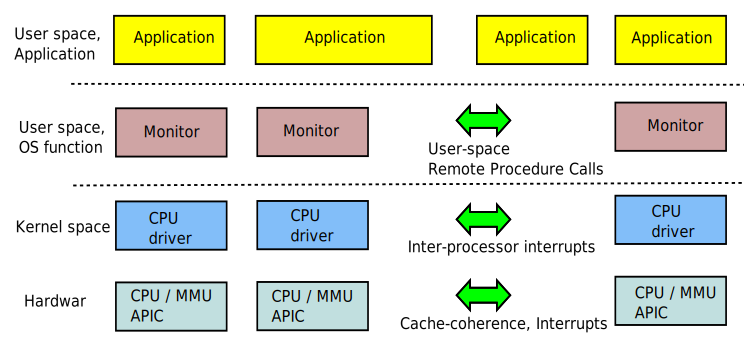
\includegraphics[width=1\textwidth]{fig/multikernel/multikernel}
    \caption{Barrelfish 구조}
  \label{fig:Barrelfish}
\end{figure}

%$$$$$$$$$$$$$$$$$$$$$$$$$$$$$$$$$$$$$$$$$$$$$$$$$$$$$$$$$$$$$$$$$$$$$$$$$$$$$$$$
%Paragraph : Barrelfish의 구조의 단점
%$$$$$$$$$$$$$$$$$$$$$$$$$$$$$$$$$$$$$$$$$$$$$$$$$$$$$$$$$$$$$$$$$$$$$$$$$$$$$$$$
Barrelfish의 구조적인 철학은 공유를 최대한 줄이는 것인데, 결국 이것은 로드 밸런싱을 수행할 수 
없는 단점을 가진다. 
예를 들어 하나의 코어에 많은 스레드들이 같이 돌고 있고, 다른 코어에는 아무런 
스레드도 없는 경우 분산 시스템 처럼 수행되므로, 동적으로 스레드에 대한 정보들을 
다른 코어로 전송할 수가 없다.
즉 분산 시스템의 전형적인 단점인 로드 밸런싱이 어려우므로 응용프로그램에 따라 
로드가 한 쪽에 몰리는 경우, 느려진 코어의 일을 기다려야 하기 때문에 전체적인 
성능이 저하될 수 있다. 

\subsubsection{FusedOS}
%$$$$$$$$$$$$$$$$$$$$$$$$$$$$$$$$$$$$$$$$$$$$$$$$$$$$$$$$$$$$$$$$$$$$$$$$$$$$$$$$
%Paragraph : Fused OS의 특징 설명
%$$$$$$$$$$$$$$$$$$$$$$$$$$$$$$$$$$$$$$$$$$$$$$$$$$$$$$$$$$$$$$$$$$$$$$$$$$$$$$$$

FusedOS는 IBM 연구소에서 개발되었으며, 모노리틱 구조와 마이크로 구조의 장점을 활용한 운영체제이다.
FusedOS의 철학은 기존 연구는 대부분 경량 커널(LWK: Light-Weight Kernel) 또는 정량 커널(FWK:
Full-Weight Kernel) 둘 중 하나의 방식으로만 개발되어온 운영체제를 LWK와 FWK를 혼합하여 만든 운영체제이다.
그 이유는 FWK으로 사용하는 리눅스로 인하여 기존 반들어진 라이브러리등을 모두 재사용할 수 있기 때문이다.
또한 LWK를 통하여 FWK이 가지고 있는 근본적인 확장성 문제를 해결할 수 있다는 것과, 과학에서 사용되는 
특정한 목적으로 HPC 위에서 개발된 응용프로그램은 커널의 간섭이 없는 LWK에서 더 효율적으로 동작하기 때문이다. 
 
\begin{figure}[h!]
    \centering
    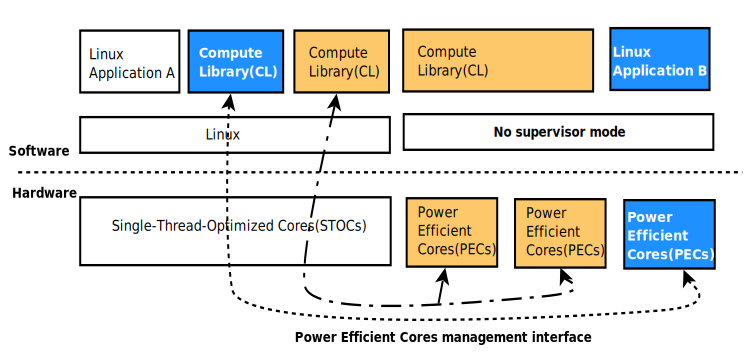
\includegraphics[width=1\textwidth]{fig/fusedos/fusedos}
    \caption{FusedOS 구조}
  \label{fig:FusedOS}
\end{figure}

%$$$$$$$$$$$$$$$$$$$$$$$$$$$$$$$$$$$$$$$$$$$$$$$$$$$$$$$$$$$$$$$$$$$$$$$$$$$$$$$$
%Paragraph : Fused OS의 구조 설명
%$$$$$$$$$$$$$$$$$$$$$$$$$$$$$$$$$$$$$$$$$$$$$$$$$$$$$$$$$$$$$$$$$$$$$$$$$$$$$$$$
이러한 FusedOS의 구조는 그림~\ref{fig:FusedOS}와 같다. 
그림과 같이 FusedOS의 하드웨어는 성능 좋은 코어 그룹(STOCs: Single-Thread-Optimized Cores)와
전력에 효율적인 코어 그룹(PECs: Power Efficient Cores)로 구성되어 있다.
PEC는 STOC의 기능 중 하나이고 superviosr 모드를 포함하고 있지 않는다. 
STOC에는 리눅스 운영체제가 동작하고, 리눅스에 기능을 추가하여 Compute Library(CL)이 PEC에 
접근이 가능하도록 설계되었다.

CL은 마치 리눅스 응용프로그램으로 동작하며, 실행을 하면 가벼운 커널을 PEC 메모리에 
전달되고 그 후 가벼운 커널은 PEC코어에서 동작한다.
이를 통해, HPC 응용의 성능을 보여주면서 리눅스 운영체제의 기능을 
제공할 수 있는 장점을 가진다. 
FusedOS의 성능은 HPC 운영체제 코어와 연산을 위한 코어가 분리되었기 때문에, 운영체제의 
방해를 받지 않아 기존 리눅스보다 높은 성능을 보인다.
이것은 기존 운영체제의 병목현상 때문에 발생하는 확장서을 문제를 해결할 수 있다.   
하지만 FusedOS 역시 독립적으로 코어에 LWK를 할당하여 호출하는 방법을 사용하므로,  
응용프로그램을 실행하고 종료하는데 추가적인 시간이 필요하다. 

\subsection{기존 운영체제 최적화}

\subsubsection{Linux scalability}

MIT PDOS 연구 그룹은 새로운 운영체제가 아닌 리눅스 커널을 대상으로 매니코어 환경에서 확장성을 연구하였다.
실제 사용되는 7가지의 응용프로그램(Exim, memcached, Apache, PostgreSQL, gmake, Psearchy, and
MapReduce)을 가지고 MOSBENCH라는 응용프로그램 벤치마크를 만들어 리눅스 커널을 
대상으로 성능을 측정하였고, 측정 중 발생되는 여러 문제를 해결하여 리눅스 커널의 확장성을 향상시켰다.

\begin{figure}[h!]
    \centering
    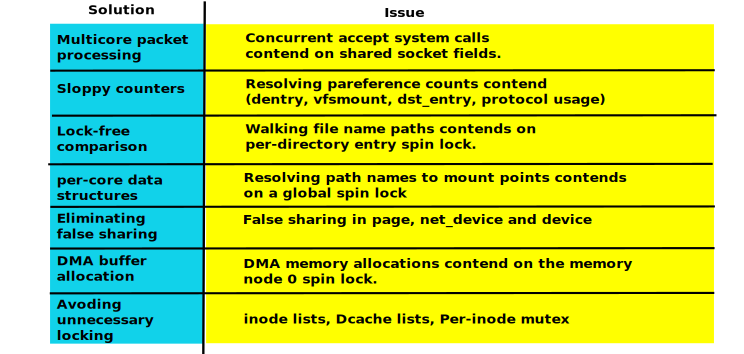
\includegraphics[width=1\textwidth]{fig/linux/linux}
    \caption{linux scalability 분석 연구}
  \label{fig:linux}
\end{figure}


그림~\ref{fig:linux}와 같이 총 7가지의 기술을 활용과 응용프로그램을 직접 수정하여 커널 확장성을 개선하였다.
먼저 멀티코어 패킷 프로세싱이 있다. 
리눅스 커널은 네트워크 멀티코어 패킷을 위해 멀티 큐를 사용하여 성능이 향상되었으나, 만약 클라이언트 
연결 주기가 짧을 경우 이러한 패킷 커넥션이 성능을 저해한다.
따라서 이 연구 그룹은 동시 다발적으로 연결을 요청하는 Apache 응용프로그램과 같은 경우는 
커널의 소켓 함수 중 accpet을 수정하여 per-core 큐에 저장하도록 수정하였다. 
이 것은 싱글 listening 소켓을 보호하기 위한 락을 제거할 수 있어 확장성을 향상시킨다.

다음으로 이 연구 그룹은 리눅스의 레퍼런스 카운트 때문에 발생하는 캐시 일관성 트래픽을 제거하기 위한 
sloppy counter를 만들었다. 
이것을 통해, 디렉토리 엔트리 오브젝트(\code{dentrys}), 마운트된 파일 시스템 오브젝트(\code{vfsmounts}) 그리고 
네트워크 프로토콜에서의 메모리 할당을 추적하기 위한 전역 변수를 sloppy counter로 수정하여 성능을 향상 시켰다. 
또한, 리눅스 커널은 디렉토리 엔트리 캐시의 이름을 찾는 부분에 \code{per-dentry} spin lock 때문에 문제가 있다. 
이러한 문제를 해결하기 위해 리눅스의 lock-free page cache lookup protocol과 유사한 방법을 활용하여 전역 spin
lock을 제거하여 성능을 향상 시켰다. 
또한 per-core 방법을 사용한 방법과 캐시라인의 false sharing때문에 발생하는 성능 저하 문제, 이더넷 디바이스 
DMA 버퍼가 한쪽 노드에만 할당되어 발생하는 확장성 문제와 그리고 불필요한 락을 제거하여 리눅스 커널의 확장성을 
향상 시켰다.  
\subsubsection{BonsaiVM}

%$$$$$$$$$$$$$$$$$$$$$$$$$$$$$$$$$$$$$$$$$$$$$$$$$$$$$$$$$$$$$$$$$$$$$$$$$$$$$$$$
%Paragraph : BonsaiVM 특징 설명
%$$$$$$$$$$$$$$$$$$$$$$$$$$$$$$$$$$$$$$$$$$$$$$$$$$$$$$$$$$$$$$$$$$$$$$$$$$$$$$$$
BonsaiVM은 MIT Parallel and Distributed Operating Systems Group에서 개발한 리눅스 커널을 위한 
가상 메모리 시스템이다. 
리눅스의 멀티 스레드들은 하나의 address space를 공유하게 되는데, 이러한 공유된 address space 때문에 
mmap과 soft page fault간에 공유된 address space를 보호하기 위해, reader-writer 세마포어를 사용한다. 
하지만, 많은 락 경합 때문에 스레들이 블락 걸리는 현상이 많이 생기는데, 이 때문에 코어가 많아 지면 성능이 떨어지는 
문제가 있다.

\begin{figure}[h!]
    \centering
    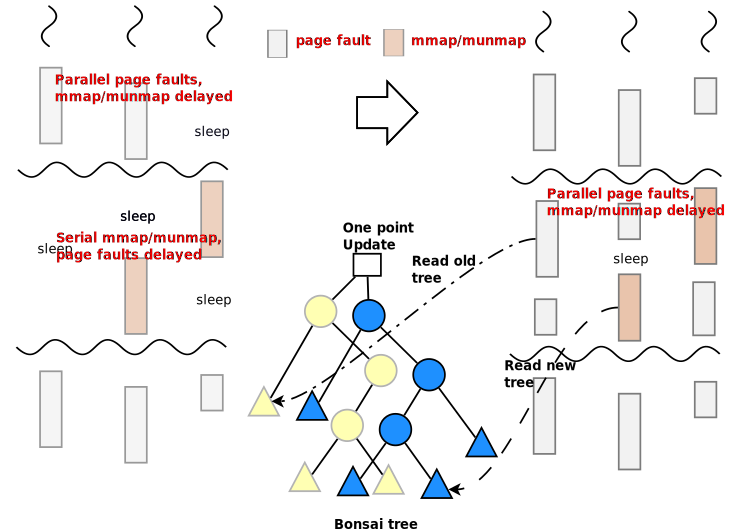
\includegraphics[width=1\textwidth]{fig/bosaivm/bosaivm}
    \caption{Address space 문제와 BosaiVM을 이용한 해결}
  \label{fig:bonsaivm}
\end{figure}

그림~\ref{fig:bonsaivm}의 왼쪽 부분은 이러한 address space를 문제를 보여준다. 
병렬로 수행이 가능한 페이지 폴트 때문에 mmap/munmap 함수는 블락이 걸리고, 병렬로 
수행이 불가능한 mmap/munmap 함수가 수행되면 mmap/munmap 함수뿐만 아니라 페이지 폴트까지 블락에 걸린다.
이러한 single address space 문제해결하기 위해서 앞에서 설명한 corey 운영체제를 만드는 등 여러 연구들이 
진행되었지만, 이 연구에서는 새로운 운영체제가 아닌 리눅스 커널을 대상으로 RCU라는 리눅스 커널의 동기화
기법을 사용하여 이 문제를 해결하였다. 
이것은 새로운 운영체제를 제안하는 것이 아니라, 리눅스 커널을 대상으로 개선한 연구이며, 리눅스 커널 중 상당히 
복잡한 가상 메모리 시스템에 직접 RCU라는 동기화 기법을 사용하여, 성능 확장성을 향상시킨 연구이다.
 
BonsaiVM은 총 3가지 기법(fault locking, hybrid locking/RCU, pure RCU)을 통해 single
address space 문제를 해결하였다.
이 중 앞의 두가지 방법은 리눅스 커널의 구현 의존 적인 해결방법이고, pure RCU는 
기존 리눅스 커널의 레드-블랙 트리를 사용하지 않고 RCU를 사용할 수 있는 
새로운 Bonsai 트리 자료구조를 만들어 문제를 해결한 방법이다. 
Bonsai 트리는 그림~\ref{fig:bonsaivm}과 같이 이진 트리로 구성되어 있으며, 
가장 큰 특징은 루트 노드의 업데이트가 원자적 명령으로 한번에 할 수 있다는 것이다. 
그 이유는 Bonsai 트리는 함수형 트리 형식으로 개발되어서, 밸런스를 수행하는 동안에도 리더들은 
old 트리의 값을 읽으며 수행할 수 있다. 
하지만 병렬로 수행할 수 있는 장점은 있지만, 트리 검색에 기존 레드-블랙 트리에 비해 많은 성능 
오버헤드가 존재하여, 실제 리눅스 커널에 적용되지는 못하였다. 
 
%$$$$$$$$$$$$$$$$$$$$$$$$$$$$$$$$$$$$$$$$$$$$$$$$$$$$$$$$$$$$$$$$$$$$$$$$$$$$$$$$
%Paragraph 2: 기법 설명
%$$$$$$$$$$$$$$$$$$$$$$$$$$$$$$$$$$$$$$$$$$$$$$$$$$$$$$$$$$$$$$$$$$$$$$$$$$$$$$$$

\subsubsection{RadixVM}

%$$$$$$$$$$$$$$$$$$$$$$$$$$$$$$$$$$$$$$$$$$$$$$$$$$$$$$$$$$$$$$$$$$$$$$$$$$$$$$$$
%Paragraph : RadixVM 특징 설명
%$$$$$$$$$$$$$$$$$$$$$$$$$$$$$$$$$$$$$$$$$$$$$$$$$$$$$$$$$$$$$$$$$$$$$$$$$$$$$$$$
RadixVM은 single address space 때문에 발생하는 확장성 문제를 해결하기 위해, 
기존 연구를 위해 개발된 운영체제를 대상으로 가상 메모리에 대한 부분을 수정하여 문제를 해결한 연구이다.
그 이유는 리눅스의 가상 메모리를 수정하는 것은 굉잡히 복잡하여, 적용하기 힘들기 떄문에 
덜 복잡한 운영체제에 새로운 개념을 적용하였다. 
RadixVM은 BonsaiVM과 같이 VM의 공유되는 adress space가 map, unmap, page fault 함수 들로 인해 
서로 경쟁함으로 발생하는 문제를 새로운 3가지 접근을 통해 해결하였다. 


  
\begin{figure}[h!]
    \centering
    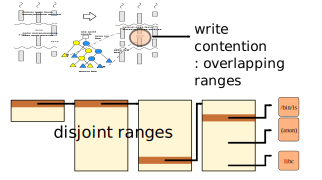
\includegraphics[width=1\textwidth]{fig/radix/radix}
    \caption{RadixVM의 해결 방법}
  \label{fig:radix}
\end{figure}


%$$$$$$$$$$$$$$$$$$$$$$$$$$$$$$$$$$$$$$$$$$$$$$$$$$$$$$$$$$$$$$$$$$$$$$$$$$$$$$$$
%Paragraph : RadixVM  기법 설명 - 1
%$$$$$$$$$$$$$$$$$$$$$$$$$$$$$$$$$$$$$$$$$$$$$$$$$$$$$$$$$$$$$$$$$$$$$$$$$$$$$$$$
첫째로, 성능 좋은 밸런스 트리를 사용하지 않고, radix 트리를 이용하는 것이다. 
RadixVM의 궁극적인 목적은 VM과 관련된 operation에 대해서는 최대한 공유를 피하자는 것이다.
만약 모든 메모리 맵을 배열로서 만들면 모든 VM관련 명령들이 충돌이 일어나지 않는다. 
하지만 이러한 방법은 너무 많은 메모리 사용량이 요구된다.
이러한 문제를 해결하기 위한 가장 좋은 방법은 하드웨어 페이지 테이블처럼 동작하는 radix 트리를 
이용하는 것이다. 
radix 트리는 트리의 읽기와 쓰기를 서로 다른 부분에 접근하도록 만들어 준다.
따라서, 배열을 사용한 방법과 같이 충돌 없이 사용가능하므로 동시에 여러 스레들이 접근 할 수 있을 뿐만아니라 
메모리 사용량도 밸런스 트리와 비슷한 수준을 유지 할 수 있다.

%$$$$$$$$$$$$$$$$$$$$$$$$$$$$$$$$$$$$$$$$$$$$$$$$$$$$$$$$$$$$$$$$$$$$$$$$$$$$$$$$
%Paragraph : RadixVM  기법 설명 - 2
%$$$$$$$$$$$$$$$$$$$$$$$$$$$$$$$$$$$$$$$$$$$$$$$$$$$$$$$$$$$$$$$$$$$$$$$$$$$$$$$
두번째 기법은 munmap할 때 발생하는 TLB shutdown 문제이다.
unmap 함수는 반드시 어떠한 코어의 페이지도 매핑이 안된 상태로 끝나야 한다.
따라서 unmap 함수는 모든 코어에 TLB shutdonw 메시지를 남기며, 이로인해 
코어가 증가 할 수록 TLB shutdown이 많이 발생하게 된다. 
radixVM에서는 이러한 문제를 per-core 페이지 테이블을 이용하여 해결하였다. 


%$$$$$$$$$$$$$$$$$$$$$$$$$$$$$$$$$$$$$$$$$$$$$$$$$$$$$$$$$$$$$$$$$$$$$$$$$$$$$$$$
%Paragraph : RadixVM  기법 설명 - 2
%$$$$$$$$$$$$$$$$$$$$$$$$$$$$$$$$$$$$$$$$$$$$$$$$$$$$$$$$$$$$$$$$$$$$$$$$$$$$$$$
RadixVM의 마지막 기법은 새로운 refcache라는 레퍼런스 카운터를 제공한다는 것이다.
레퍼런스 카운터는 최근 운영체제의 가장 큰 확장성 저해요소 중에 하나이다.
이러한 레퍼런스 카운터는 3가지 종류로 개발되고 있다. 먼저 가장 쉬운 방법인 락을 
이용하는 방법이 있다. 즉 모든 증가/감소 명령의 앞뒤에 락을 호출하는 것이다. 
이것은 락 때문에 상당히 많은 캐시-라인 경합이 발생된다. 
다른 방법으로는 원자적 증가/감소 명령을 이용하는 것이다. 하지만 이러한 방법도 결국 
전역 변수 때문에 캐시-라인 경합이 발생한다. 
최근의 방법으로는 per-core 카운터를 이용하는 것이다. 
하지만, 단순히 per-core 카운터를 이용하는 것은 코어 수에 비례하여 공간에 대한 오버헤드를 가지게 된다.
RadixVM은 이러한 확장성과 메모리 사용량에 대한 오버헤드를 동시에 줄이기 위해, 
10ms의 시간(epochs)을 기반으로 per-core에 저장된 델타 카운트를 
체크하여 전역 카운터에 적용하는 방법을 사용하였다.

\subsubsection{SC rule}

%$$$$$$$$$$$$$$$$$$$$$$$$$$$$$$$$$$$$$$$$$$$$$$$$$$$$$$$$$$$$$$$$$$$$$$$$$$$$$$$$
%Paragraph : SC rule 특징 및 역사 설명 
%$$$$$$$$$$$$$$$$$$$$$$$$$$$$$$$$$$$$$$$$$$$$$$$$$$$$$$$$$$$$$$$$$$$$$$$$$$$$$$$$
SC rule은 MIT  PDOS 연구 그룹에서 연구한 운영체제의 확장성 개선을 새로운 관점으로 바라본 연구이다. 
기존 연구들은 대부분 운영체제의 병목지점을 추출한 후 이러한 병목지점을 해결하기 위해 새로운 
동기화 기법을 개발하거나 기존 개발된 동기화 기법을 적용하는 방법을 사용하였다. 하지만, 이러한 방법들은 
모두 워크로드가 다름에 따라 서로 다른 양상을 가지고, 
또한 문제를 해결하는데 너무 오랜시간이 걸리는 문제점을 가지고 있다.
실제 확장성에 대한 문제는, 대부분 설계 단계에서 인터페이스를 확장성 있게 소프트웨어를 설계하면 해결된다는 것이다. 
이러한 가정을 가지고 확장성을 위해서는 확장성있는 설계가 중요하며 그에 대해서 초점을 둔 논문이다.
그 이유는 리눅스등의 운영체제는 확장성 있게 설계 되었으나 응용프로그램의 사용방법에 따라 확장성 문제가 발생하기 
때문이다.
예를 들어 원작적으로 값 X를 변수 A에 추가하고, 다른 CPU가 원자적으로 같은 변수에 Y라는 값을 추가하였다면, 
두 가지의 명령의 순서는 상관 없고, 결국에는 X + Y의 값이 변수 A에 저장된다는 것이다.
또한, SC rule은 이러한 문제점을 발견하기 위해 메모리의 충돌을 발견하는 새로운 툴을 제안하였다. 
이러한 툴을 통해 설계 단계에서 확장성 문제를 발견할 수 있으며, 이 툴을 통해 기존 운영체제(리눅스, sv6)의 
문제점을 분석하였다. 

%$$$$$$$$$$$$$$$$$$$$$$$$$$$$$$$$$$$$$$$$$$$$$$$$$$$$$$$$$$$$$$$$$$$$$$$$$$$$$$$$
%Paragraph : SC rule 예제 설명 
%$$$$$$$$$$$$$$$$$$$$$$$$$$$$$$$$$$$$$$$$$$$$$$$$$$$$$$$$$$$$$$$$$$$$$$$$$$$$$$$$
저자는 POSIX의 오퍼레이션들은 가환성(commutativity)이 있지 않고, POSIX 오퍼레이션들을 
확장성 있게 만드는 것은 어렵다.
하나의 예로 프로세스를 복사하는 \code{fork()}는 가환성을 가지고 있지 않다. 
하지만 저자는 \code{fork()}를 \code{posix\_spawn()}으로 수정하면 가환성을 가지게 되고, 이것은 결국 
확장성을 향상시키게 된다.  
또한 \code{open()}는 사용가능한 낮은 숫자부터 반환하게 되는데 이것을 \code{open()}과 \code{O\_ANYFD}을 함께
사용하면 가한성을 있게 만들 수 있다고 제안하였다.
이처럼 리눅스 커널은 가환성을 잘 지키도록 호출 해주면, 확장성을 향상 시킬 수 있고 이것은 설계단계에서 
처리할 수 있다는 것이다.
저자는 QEMU을 수정하여 리눅스의 가환성을 분석 할 수 있는 Commuter라는 툴을 제공한다. 

